\documentclass[11pt,a4paper]{article}
\usepackage[T1]{fontenc}
\usepackage{lmodern}
\usepackage[margin=22mm]{geometry}
\usepackage{graphicx,booktabs,amsmath,amssymb,array,tabularx,longtable}
\usepackage{enumitem,float}
\usepackage{microtype,needspace}
\usepackage[hidelinks]{hyperref}
\usepackage{url}
\graphicspath{{figures/}}
\setlength{\parindent}{0pt}
\setlength{\parskip}{5pt}
\setlength{\textfloatsep}{9pt}
\setlength{\intextsep}{9pt}
\setlength{\tabcolsep}{5pt}
\setlength{\emergencystretch}{1em}
\renewcommand{\arraystretch}{1.12}
\renewcommand{\thesection}{S\arabic{section}}
\renewcommand{\thefigure}{S\arabic{figure}}
\renewcommand{\thetable}{S\arabic{table}}
\renewcommand{\theequation}{S\arabic{equation}}
\newcolumntype{Y}{>{\raggedright\arraybackslash}X}
\newcommand{\Normal}{Normal}
\newcommand{\Compact}{Compact}
\newcommand{\June}{June}
\newcommand{\repo}[1]{\path{#1}}
\begin{document}
\begin{center}
{\Large\bfseries Supplementary Material\par}
\vspace{5pt}
{\large\bfseries FCNPilot: A Tool-Grounded Agentic Framework for End-to-End Field-Coupled Nanocomputing Circuit Design\par}
\end{center}

\Needspace{4\baselineskip}
\section{Benchmark identity and supported circuit semantics}
The experimental unit is a frozen circuit representation, not a filename presumed to denote a standard function. The corpus contains 17 TOY and 13 MAJ representations. Exact-byte identity and complete Boolean-function identity are reported separately (Figure~\ref{fig:curation}). The 16 function groups retain the declared input/output ordering; they are not equivalence classes under arbitrary port permutations or negation--permutation transformations. One representative per group was fixed in the manifest before backend comparison.

\begin{figure}[htbp]
\centering
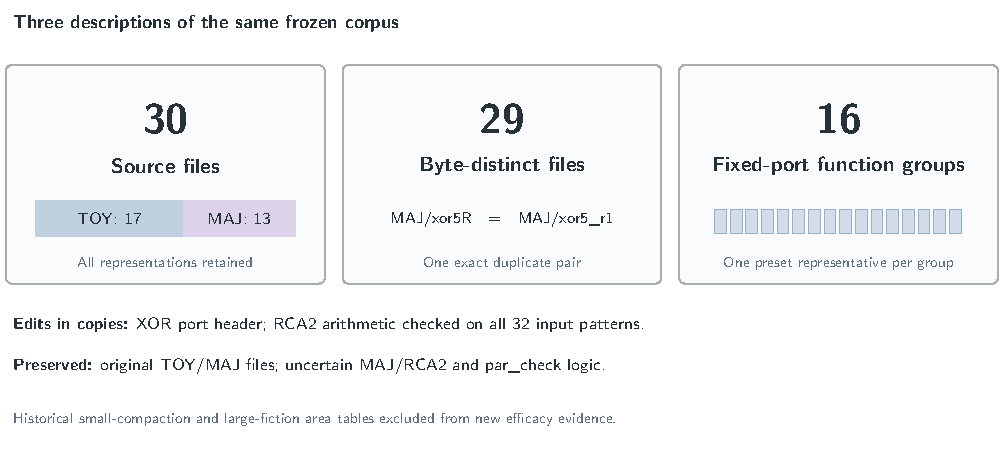
\includegraphics[width=\linewidth]{figS1_benchmark_curation.pdf}
\caption{Three descriptions of one frozen corpus: 30 representations (17 TOY, 13 MAJ), 29 byte-distinct files, and 16 truth-table groups under fixed declared port order. These are not sequential filtering steps. MAJ/xor5R and MAJ/xor5\_r1 are the sole byte-identical pair. Only frozen copies are corrected: the TOY/xor2 port header and two TOY/RCA2 carry expressions; the latter passes an independent arithmetic reference on all 32 vectors. Original files are preserved. MAJ/RCA2 and par\_check retain their source logic, and historical area tables excluded by the eligibility manifest are not new efficacy evidence. AI assistance was used to prepare the TikZ code; the corpus counts derive from the archived manifest.}
\label{fig:curation}
\end{figure}

The supported source language consists of one scalar combinational module with explicit input, output, and wire declarations and single-driver continuous assignments. Scalar ANSI and non-ANSI port declarations are accepted. Expressions contain signal names, parentheses, complement, AND, OR, and XOR. XOR is lowered to an AND/OR/inverter expression for the existing parsers. Undeclared or undriven signals, multiple drivers, and combinational cycles are rejected. Constants, buses, hierarchical instances, procedural blocks, and state elements are outside this implementation. A retained legacy header discrepancy is disclosed, with the declaration lists defining the audited interface; this convention is not a claim of full Verilog language conformance.

All 30 frozen inputs passed the recorded Yosys parsing check and the source-to-normalized-expression comparison. The two TOY/RCA2 corrections concern low-bit carry generation and use of the intermediate carry. Its reference is integer two-bit unsigned addition with carry-in, not a second evaluation of the same source expressions. Conversely, the single output of 1bitAdderMaj is described by its actual majority network, not presumed to be a complete full adder.

\Needspace{4\baselineskip}
\section{Acceptance conditions and finite candidate selection}
Let $S$ have $n$ declared inputs and $m$ outputs. A candidate $c_j$ comprises its actual routed DAG $G_j$, placement, routes, phases, and mapped QCA artifact $Q_j$. Define $D_j$ as the implemented structural/geometric checks, $C_j$ as the applicable clock checks, and $M_j$ as successful native mapping and crossover validation. These are separate conditions on different representations, not statistically independent events. The terminal condition is
\begin{equation}
 I_j=[|Q_j|>0]\land[|\operatorname{PI}(Q_j)|=n]
                  \land[|\operatorname{PO}(Q_j)|=m].
\end{equation}
This is a cardinality condition on cell-function labels. It does not establish a name-preserving or signal-preserving bijection between QCA terminals and source ports.

For $1\le n\le11$, the source and DAG are evaluated for every input vector. DAG inputs require exact names; outputs require exact names or an explicit pure-signal alias chain in the source, and the resulting output mapping must be bijective. Missing metadata, unsupported gate semantics, and ambiguous ports return unsupported rather than pass. With $\beta_j$ denoting this explicit binding, the production acceptance rule is
\begin{equation}
 A_j=D_j\land C_j\land M_j\land I_j\land L_j,\qquad
 L_j=\begin{cases}
 [F_S(x)=F_{G_j,\beta_j}(x)\ \forall x\in\{0,1\}^n],&1\le n\le11,\\
 [\text{input-limit exemption recorded}],&n>11.
 \end{cases}
\end{equation}
The latter branch explicitly records that Boolean verification was not performed. It is not an equivalence result. Other unsupported results are rejected. Audited DAG semantics comprise binary AND/OR, unary NOT and identity nodes, and three-input majority, with explicit arity checks and non-inverting edges.

\textbf{Candidate-selection procedure.} The ordered available set is Normal, Compact, June in automatic mode, or the explicitly requested backend alone. Let its size be $K\le3$ and let $t_0$ be the start of the P\&R selection stage.
\begin{enumerate}[leftmargin=18pt,itemsep=1pt,parsep=0pt,topsep=4pt]
\item For each untried backend $j$, abort on cancellation. Compute $r=T-(t-t_0)$. If $r<1$ second, record budget exhaustion and skip the call.
\item Allocate $b_j=\max(1,\lfloor r/(K-j+1)\rfloor)$ seconds. Create a fresh candidate directory and run the backend with an external-call timeout $b_j$; its internal budget is capped at $\min(240,\max(1,b_j-2))$ seconds.
\item Require the requested backend identity and successful structural, geometric, clock, and native mapping checks. Evaluate the source/DAG condition above against the original source snapshot.
\item Subtract elapsed candidate time from $b_j$. Reject if no time remains; otherwise map the candidate to QCA using that remaining external-call allowance and check $I_j$.
\item If accepted, preserve the artifacts and return the candidate immediately. On error or timeout, preserve the rejection evidence; automatic mode advances once, whereas an explicitly requested backend fails. If none is accepted, the stage fails.
\end{enumerate}

For each routed adjacency, the common clock test is $\Delta\phi\bmod4\in\{0,1\}$ with four valid phases. Normal additionally checks the fixed 2DDWave template and left/top gate-entry directions. Same-phase progression is allowed in irregular layouts. The checks do not prove equal fanin arrival cycles, physical settling, or waveform correctness. Reported maximum same-phase runs are not a universal acceptance bound shared by all three backends.

One invocation starts at most $K$ backends because it traverses a finite list without returning to an earlier candidate. Under finite local checks and normal process termination it terminates; it has no area-optimality guarantee. $T$ governs P\&R selection, not the entire design flow, and is not a hard real-time bound: process polling, termination grace, local verification, and artifact handling add overhead. A user-requested resume creates another stage attempt, so the bound does not apply cumulatively across repeated resumes.

\Needspace{4\baselineskip}
\section{Protocols and separation of experimental versions}
The backend matrix, language-agent pilot, and later guarded-production checks answer different questions. Their immutable protocol files and per-run artifacts define the experimental versions; no unrecorded software release or model-weight revision is inferred from a directory name.

\begin{table}[H]
\centering
\caption{Recorded experimental controls. Time budgets refer to their stated scope.}
\begin{tabularx}{\linewidth}{@{}p{29mm}YYY@{}}
\toprule
Control & Backend matrix & Language-agent pilot & Later XOR checks\\
\midrule
Design & 30 representations $\times$ 3 explicit backends & 4 tasks $\times$ 2 repeats $\times$ 3 methods & One frozen XOR; 3 backends\\
Endpoint & Device mapping & Device mapping & Both simulation models and standard energy\\
Budget & 180 s per backend command & 180 s per trial; backend 90 s & Initial 180 s; separate June follow-up 600 s\\
Concurrency & 2 & 2 & Shared-host validation, not a speed experiment\\
Seed & Recorded seed 1 & Backend seed 1; schedule seed 20260905 & Recorded seed 1\\
Failures & One run per input/backend; no retry replacement & Fresh sessions; every service failure retained & Initial June timeout retained\\
\bottomrule
\end{tabularx}
\label{tab:protocols}
\end{table}

\textbf{Frozen backend matrix.} Ninety runs were scheduled through mapping, with no LLM in the loop. A nominal Bistable model and 512 samples were recorded in the common configuration but no simulation or energy stage was requested. Normal exposes seed control; native Compact and June do not expose their internal seed, so recording seed 1 does not establish identical control of native randomness. Normal may canonicalize an equivalent parity expression, and the backends may retain different buffer nodes. Consequently this is a comparison of complete source-to-layout flows, not identical-DAG placement algorithms. Shared-host wall times are not isolated speed measurements.

The original execution criterion gave 21, 10, and 24 completions for Normal, Compact, and June. Subsequent audit of these same artifacts found 51 Boolean-equivalent DAGs, four unsupported audits, and no established Boolean counterexample among the 55 completed runs. Terminal counts excluded four results, one already excluded by the logic audit. Thus 48/90 met both added qualifications: 16/30, 9/30, and 23/30. For the preselected function representatives the counts were 8/16, 5/16, and 13/16. Area comparisons use the same-input intersection passing the stated checks, not unmatched successful subsets.

These are retrospective qualifications of the frozen matrix. The production implementation subsequently incorporated logic and terminal checks into candidate selection, but the entire 90-run matrix was not rerun. Current guarded acceptance must therefore not be assigned a prospective 48/90 success rate. In later tests, MAJ/clpl was rejected by Normal for a missing explicit output binding, Compact exhausted its 77-second native routing budget, and June preserved five output terminals. TOY/clpl passed source/DAG logic with all three backends but each device had only one of five declared outputs, so all were rejected.

\textbf{Language-agent pilot.} The tasks were ordinary XOR mapping; explicitly requested Compact mapping of MAJ/1bitAdderMaj; recovery from a nonexistent input using a supplied valid fallback; and mux21 mapping with specified artifact reads. The two LLM methods used the same configured identifier \texttt{qwen3-vl-plus}, tools, task prompts, and limits: 12 tool calls and 3500 output tokens per trial. Only the system prompt differed. The fixed script received structured task fields and a predefined recovery policy; it did not perform natural-language interpretation. Trial order was shuffled with a recorded seed; failures were not rerun, and no LLM judge was used.

Actual mapping completed in 8/8 script, 7/8 generic-Pi, and 6/8 domain-agent trials. Prespecified structured delivery passed 8/8, 5/8, and 6/8; an additional disclosed prose audit yielded 8/8, 5/8, and 5/8. Each LLM condition encountered one connection failure and one account-status refusal. These infrastructure events do not establish capability differences. Prompt changes made after the pilot, including stronger unit and provenance rules, were not retested with an LLM. The small pilot establishes neither prompt superiority nor generalization to unrestricted circuit design.

\Needspace{4\baselineskip}
\section{XOR numerical diagnostics and their limits}
The later checks used the same frozen scalar XOR source and executed both Bistable and Coherence numerical implementations before standard energy analysis. Normal produced 12 tiles and 79 QCA cells; Compact 24 tiles and 119 cells; and June 65 tiles and 214 cells. The Normal device contains 72, two, and five cells on its three layers. Tile area and device-cell count are distinct quantities. June's successful full flow is the separately recorded 600-second-budget follow-up; its initial 180-second energy-stage timeout remains a failed trial.

\begin{figure}[htbp]
\centering
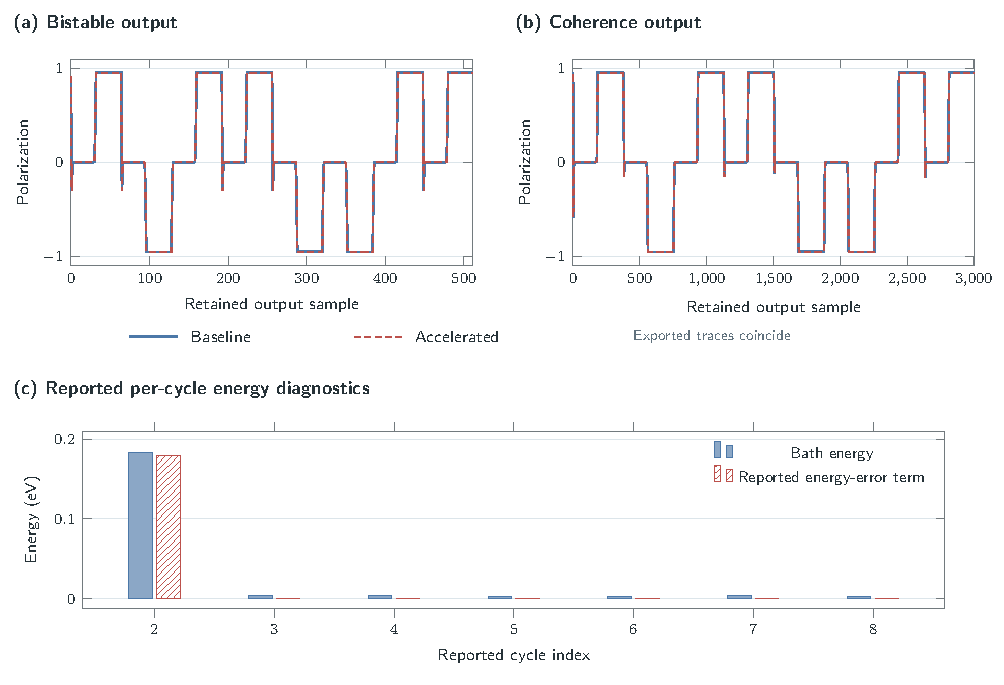
\includegraphics[width=\linewidth]{figS2_numerical_diagnostics.pdf}
\caption{Diagnostics for the Normal XOR in main-text Figure 3. (a,b) All 512 Bistable and 3005 retained Coherence samples are plotted without resampling or realignment. Coincident baseline/accelerated traces test implementation agreement, not source-to-device behavior; the abscissa is retained sample index. (c) All seven reported energy cycles are retained, including the large initial energy-error diagnostic, which is not a statistical error bar. Energy and Coherence steps are $10^{-17}$ and $10^{-16}$ s, respectively. No time-step or steady-state convergence is established. AI assistance was used to prepare the TikZ plotting code; all plotted values come from archived numerical outputs.}
\label{fig:numerics}
\end{figure}

The Normal Coherence calculation records 700000 integration steps over $7\times10^{-11}$ s, while its exported output contains 3005 retained samples. The plots use every retained value, not every internal step. Baseline and accelerated output arrays are identical in the archived serialization. Normal's Bistable comparison reports zero samples at the 100-iteration limit; Compact reports seven such samples despite numerical-engine agreement and is consequently completed with warnings. Agreement between implementations is not a convergence test or a source-to-device waveform proof.

Standard energy analysis uses a $10^{-17}$ s step, $8\times10^{-11}$ s duration, and $10^{-11}$ s clock period. The seven reported cycle indices are 2--8. Normal's first reported cycle has bath energy 0.182791 eV and energy-error term 0.179875 eV; its seven-cycle mean bath energy is 0.0289886 eV. These values retain the initial transient rather than selecting only the smaller later cycles. Dividing mean bath energy by clock period, with the eV-to-joule conversion, defines a model power estimate; it does not establish converged dissipated power. The signed bath-plus-clock quantity is an energy-balance diagnostic and must not be interpreted as total-chip power. Preview mode has a larger $2\times10^{-15}$ s step and is not used for Figure~\ref{fig:numerics}.

\Needspace{4\baselineskip}
\section{Evidence assets and reproducibility boundaries}
The paper's local \repo{paper/data/} directory contains the tabulated figure data and the archived \repo{device_runs/} artifacts used for the XOR illustrations. Each algorithm's provenance receipt records the original run, original manifest digest, artifact identity, and SHA-256 digest. The XOR snapshots include the source, normalized source, routed DAG, IFCN layout, mapped QCA device, logic and interface reports, numerical traces, and energy reports. Figure sidecars connect the rendered claims to these artifacts. Regenerating a drawing reads archived coordinates or values; it does not rerun a placement algorithm or simulator.

Table~\ref{tab:assets} identifies the broader research assets by paths relative to the FCNPilot repository. These paths distinguish the full experimental archive from the smaller figure-data copy in the manuscript directory. Recorded paths and digests retain historical provenance; analysis scripts resolve local copies. Machine-specific binaries, shared libraries, font caches, locks, and redundant previews are excluded. Their fingerprints remain, but reproducing the historical runtime requires rebuilding or supplying its dependencies. Consolidation does not imply a rerun with current source.

\begin{table}[H]
\centering
\caption{Research assets and the claims they permit checking. Paths are relative to the FCNPilot repository unless otherwise stated.}
\begin{tabularx}{\linewidth}{@{}p{31mm}Y@{}}
\toprule
Asset & Location and purpose\\
\midrule
Frozen corpus & \repo{engine/tests/benchmarks_pi/v1/manifest.json}: original and frozen input digests, declared interfaces, corrections, truth-table groups, and preselected representatives. \repo{evidence_eligibility.json} in the same directory separates eligible and excluded historical material.\\
Backend experiment & \repo{experiments/archive/backend/}: protocol, complete runs, results, summaries, and implementation/runtime fingerprints. The summaries retain original execution outcomes and separate retrospective qualifications.\\
Language experiment & \repo{experiments/archive/pilot/}: protocol, effective prompts, requests, tool traces, final answers, machine checks, original aggregation, and post-hoc text audit.\\
Later production checks & \repo{experiments/archive/production/release-logic-io-20260905T110234Z/} and \repo{experiments/archive/production/release-logic-io-20260905T110907Z/}: initial checks and separate June follow-up, including the retained timeout.\\
Source/DAG audit & \repo{engine/scripts/verify_routed_logic.py}: read-only exhaustive evaluation and explicit port binding; records source/DAG digests, vector counts, unsupported reasons, and counterexamples when present.\\
Flow and geometry & \repo{engine/scripts/ifcn_agent.py}, \repo{engine/scripts/ifcn_agent_backend.py}, and \repo{engine/scripts/ifcn_agent_layout_validation.py}: stage acceptance, actual backend invocation, geometric checks, and cancellation behavior.\\
Figure provenance & \repo{paper/figures/} and \repo{paper/data/}: editable figure sources, captions, evidence sidecars, and archived data; the manuscript carries the corresponding figures and figure-data copy.\\
\bottomrule
\end{tabularx}
\label{tab:assets}
\end{table}

The frozen corpus manifest used by the 90-run protocol has SHA-256
\begin{center}\small\texttt{1da5652de065b0069d0cbd86a4b50ea7f9d380f1dc43095c72ca50f53c60afd8}.\end{center}
The common frozen XOR source has SHA-256
\begin{center}\small\texttt{83f8a5bb72512bf03fef78b22937aab8a786d5472c5efee71fdfe80d51651c55}.\end{center}
Protocol records also fingerprint the executed Python and native roles and relevant source/library files before and after the frozen experiments. These identify the tested implementation more precisely than assigning an unrecorded release label. The configured model name is recorded; an immutable provider model-weight revision was not independently established.

Rechecking artifact hashes establishes identity, not physical correctness. For functional auditing, the original source and actual routed DAG must be paired through their manifest entries, then the explicit Boolean and QCA terminal-count qualifications evaluated separately. Results rejected or unsupported at either level remain visible. Hash-verified stage reuse supports that audit trail; it does not upgrade a previous geometry-only result into functional evidence. The present reproducibility package supports inspection of limited combinational functions, mapped geometry, numerical implementation agreement, and observed agent behavior. It does not establish industrial-scale coverage, source-to-device timing equivalence, fabrication validity, or converged power accuracy.

\end{document}
